\documentclass[../mathNotesPreamble]{subfiles}

\providecommand{\relscalefact}{1.4}
\begin{document}
\relscale{\relscalefact}
  \section{6.3: Inverse Trigonometric Functions}

  %Show domain/range of sin/cos/tan
  %Describe domain/range of asin/acos/atan
  \begin{thmBox*}
    Note that $\sin(x)$ and $\cos(x)$, 
    \begin{itemize}
      \item take in the measure of an angle, and 
      \item return the ratio of the sides.
    \end{itemize}
    Recall that trigonometric functions are periodic:
    \begin{center}
      \begin{tikzpicture}[declare function={
        f(\x)=sin(deg(\x*pi));
        g(\x)=cos(deg(\x*pi));
        },
        ]
        \begin{groupplot}[
          group style={group size=2 by 1,horizontal sep=20mm},
          axis lines=center,
          axis line style={->},
          xmin=-2, xmax=2,
          xtick={-4,-3,...,4},
          xticklabels={$-4\pi$, $-3\pi$, $-2\pi$, $-\pi$, , $\pi$, $2\pi$, $3\pi$, $4\pi$},
          minor x tick num=1,
          ymin=-1, ymax=1,
          ytick={-1,0,1},
          minor y tick num=1,
          xlabel=, ylabel=,
          enlargelimits={abs=0.1},
          height=0.5*\axisdefaultheight, width=0.475\linewidth,
          ticklabel style={font=\normalsize,inner sep=5pt,fill=white,opacity=1.0, text opacity=1},
          every axis plot/.append style={domain=-4:4},
          ]
          \nextgroupplot
            \addplot[-] {f(x)};
            \addplot[-, red, line width=2pt] expression[domain=-0.5:0.5] {f(x)};
          \nextgroupplot
            \addplot[-] {g(x)};
            \addplot[-, red, line width=2pt] expression[domain=0:1] {g(x)};
        \end{groupplot}
      \end{tikzpicture}
    \end{center}
    
    Consider the following restricted domains and associated ranges:
    \begin{center}
      \begin{tabular}{@{}lcc@{}}\toprule
        & Domain& Range\\\midrule
        $y=\sin(x)$& $\sbrkt{-\frac{\pi}{2},\frac{\pi}{2}}$& $\sbrkt{-1,1}$\\[10pt]
        $y=\cos(x)$& $\sbrkt{0,\pi}$& $\sbrkt{-1,1}$\\[10pt]
        $y=\tan(x)$& $\parens{-\frac{\pi}{2},\frac{\pi}{2}}$& $\parens{-\infty, \infty}$\\
        \bottomrule
      \end{tabular}
    \end{center}
    When we use the restricted domains, then these functions are \hyperref[defn:oneToOne]{one-to-one}. The resulting inverse functions are:
    \begin{align*}
      \arcsin(y)&=\sin^{-1}(y)\\
      \arccos(y)&=\cos^{-1}(y)\\
      \arctan(y)&=\tan^{-1}(y)
    \end{align*}
  \end{thmBox*}
  \begin{ex*}
    Since $\sin\parens{0.96593}\approx\frac{5\pi}{12}$, what is $\sin^{-1}\parens{\frac{4}{15}}$?
    \vspace*{\stretch{1}}
  \end{ex*}
  \pagebreak

  %graphs - side by side sin vs asin, cos vs acos
  \begin{center}
    \begin{tikzpicture}
      \begin{groupplot}[
        group style={group size=2 by 3,horizontal sep=20mm,vertical sep=20mm},
        axis lines=center,
        axis line style={->},
        xmin=-0.5, xmax=0.5,
        xtick={-0.5,0,0.5},
        xticklabels={$-\dfrac{\pi}{2}$, , $-\dfrac{\pi}{2}$},
        minor x tick num=1,
        ymin=-1, ymax=1,
        ytick={-1,0,1},
        minor y tick num=1,
        xlabel=, ylabel=,
        enlargelimits={abs=0.1},
        height=0.8*\axisdefaultheight, width=0.45\linewidth,
        ticklabel style={font=\normalsize,inner sep=5pt,fill=white,opacity=1.0, text opacity=1},
        ]
        \nextgroupplot[title={$y=\sin(x)$},]
          \addplot[-] expression[domain=-1/2:1/2]{sin(deg(x*pi))};
        \nextgroupplot[title={$y=\sin^{-1}(x)$},
          xmin=-1, xmax=1,
          xtick={-1,0,1},
          xticklabels={-1,,1},
          ymin=-0.5, ymax=0.5, 
          ytick={-0.5,0,0.5},
          yticklabels={$-\dfrac{\pi}{2}$,,$\dfrac{\pi}{2}$},
          minor y tick num=1,
          ]          
          \addplot[-] expression[domain=-1:1]{asin(x)/180};
        \nextgroupplot[title={$y=\cos(x)$},
          xmin=0, xmax=1,
          xtick={0,0.5,1},
          xticklabels={,$\dfrac{\pi}{2}$, $\pi$}]
          \addplot[-] expression[domain=0:1]{cos(deg(x*pi))};
        \nextgroupplot[title={$y=\cos^{-1}(x)$},
          xmin=-1, xmax=1,
          xtick={-1,0,1},
          xticklabels={-1,,1},
          ymin=0, ymax=1, 
          ytick={0,0.5,1},
          yticklabels={,,$\dfrac{\pi}{2}$,$\pi$},
          minor y tick num=1,
          ]       
          \addplot[-] expression[domain=-1:1]{acos(x)/180};
        \nextgroupplot[title={$y=\tan(x)$},
          ymin=tan(deg(-0.45*pi)), ymax=tan(deg(0.45*pi)),
          ytick={-5,0,5},
          yticklabels={-5,,5},
          ]
          \addplot[-] expression[domain=-0.45:0.45]{tan(deg(x*pi))};
          \draw[dashed, black!50] (-0.5,{atan(-0.45)}) -- (-0.5,{atan(0.45)});
          \draw[dashed, black!50] (0.5,{atan(-0.45)}) -- (0.5,{atan(0.45)});
        \nextgroupplot[title={$y=\tan^{-1}(x)$},
          xmin=-6.3, xmax=6.3,
          xtick={-5,0,5},
          xticklabels={-5,,5},
          ymin=-0.5, ymax=0.5, 
          ytick={-0.5,0,0.5},
          yticklabels={$-\dfrac{\pi}{2}$,,$\dfrac{\pi}{2}$},
          minor y tick num=1,
          ]
          \addplot[-] expression[domain=-12.7:12.7]{atan(x)/180};
          \draw[dashed, black!50] ({atan(-0.45)},-0.5) -- ({atan(0.45)},-0.5);
          \draw[dashed, black!50] ({atan(-0.45)}, 0.5) -- ({atan(0.45)}, 0.5);
      \end{groupplot}
    \end{tikzpicture}
  \end{center}
  \pagebreak

  %Eval inv trig with special angles
  \begin{ex*}
    Evaluate the following:
    \begin{extasks}[after-item-skip=\stretch{1}](2)
      \task $\sin^{-1}\parens{\dfrac{\sqrt{2}}{2}}$
      \task $\cos^{-1}\parens{-\frac{1}{2}}$
      \task $\tan^{-1}\parens{-1}$
      \task $\tan^{-1}\parens{\dfrac{\sqrt{3}}{3}}$
    \end{extasks}
    \vspace*{\stretch{1}}
  \end{ex*}

  %Eval inv trig with calc from figure
  \begin{ex*}
    Use inverse trigonometric functions to solve for the following angles:
    \vspace*{\baselineskip}

    \noindent
    \begin{minipage}{0.425\linewidth}
      \begin{flushright}
        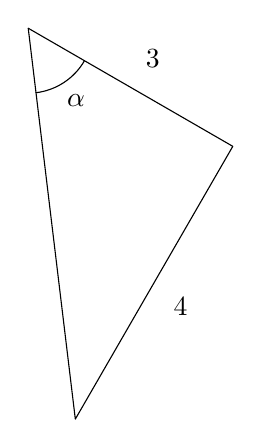
\begin{tikzpicture}[
          declare function={r=5.5; alfa=acos(3/5); d=150;},
          line cap=round, line join=round,
          ]
          %C
          %|\
          %| \
          %B--A
          %transformed using Givens: G=[[cos(d),-sin(d)],[sin(d), cos(d)]]
          \coordinate (A) at (0,0);
          \coordinate (B) at ({-3*cos(d)},{-3*sin(d)});
          \coordinate (C) at ({-3*cos(d)-4*sin(d)},{-3*sin(d)+4*cos(d)});
          \draw (A) -- node[pos=0.5, label=-90+d:$3$] {}
                (B) -- node[pos=0.5, label=180+d:$4$] {}
                (C) -- node[pos=0.5] {}
                cycle;
          %
          \tkzMarkRightAngle[size=0.4](A,B,C);
          %
          \draw[black,-] (180+d:0.15*r) arc [start angle=180+d, delta angle=-alfa, radius=0.15*r];
          \node at (180+d-alfa/2:0.2*r) {$\alpha$};
        \end{tikzpicture}
      \end{flushright}
    \end{minipage}%
    \hspace*{\stretch{1}}
    \begin{minipage}{0.425\linewidth}
      \begin{flushright}
        \begin{tikzpicture}[
          declare function={r=5.5; bta=acos(15/17); d=-45;},
          line cap=round, line join=round,
          ]
          %C
          %|\
          %| \
          %B--A
          %transformed using Givens: G=[[cos(d),-sin(d)],[sin(d), cos(d)]]
          \coordinate (A) at (0,0);
          \coordinate (B) at ({15/17*r*cos(d)},{15/17*r*sin(d)});
          \coordinate (C) at ({15/17*r*cos(d)-8/17*r*sin(d)},{15/17*r*sin(d)+8/17*r*cos(d)});
          \draw (A) -- node[pos=0.5] {}
                (B) -- node[pos=0.5, label=0+d:$4$] {}
                (C) -- node[pos=0.5, label=90+bta+d:$17$] {}
                cycle;
          %
          \tkzMarkRightAngle[size=0.4](A,B,C);
          %
          \draw[black,-] (d:0.2*r) arc [start angle=d, delta angle=bta, radius=0.2*r];
          \node at (d+bta/2:0.25*r) {$\beta$};
        \end{tikzpicture}
      \end{flushright}
    \end{minipage}%
  \end{ex*}
  \pagebreak

  %Composite (e.g. sin(atan(...)) ) sin(acos(4/5))
  \begin{ex*}
    Evaluate the following:
    \begin{extasks}[after-item-skip=\stretch{1}](2)
      \task $\sin^{-1}\parens{\sin\parens{37^\circ}}$
      \task $\cos^{-1}\parens{\cos\parens{\frac{9\pi}{4}}}$
      \task $\sin^{-1}\parens{\cos\parens{\frac{40}{41}}}$
      \task $\tan^{-1}\parens{\sin\parens{\frac{12}{20}}}$
    \end{extasks}
    \vspace*{\stretch{1}}
  \end{ex*}

  %Simplify cos(asin(x/3)), -3<=x<=3
  %Simplify sin(atan(4x)), -1/4<=x<=1/4
  \begin{ex*}
    Simplify the following:
    \begin{extasks}[after-item-skip=\stretch{1}](1)
      \task $\cos\parens{\sin^{-1}\parens{\frac{x}{3}}}$, where $-3\leq x\leq 3$
      \task $\sin\parens{\tan^{-1}\parens{4x}}$
    \end{extasks}
    \vspace*{\stretch{1}}
  \end{ex*}

  \pagebreak
\end{document}
